%% -*- coding: utf-8-unix -*-

\chapter{PoC}
\label{chap:poc}

 \section{PoCの概要}
 \label{sec:poc-overview}

 % なんのために、どういったテストをおこなうのか。
 % そもそものPoCの考え方のまとめ・整理

 % 障害報告ストーリー – NetTester
 % \url{https://3.basecamp.com/3088280/buckets/867009/documents/151143879}
 % どういったサービス上のトラブルを検出したいとおもったのか? (ユースケース例)
 % 技術的にやりたいこと:  静的なテスト/動的なテスト

 \subsection{PoCの目的}
 \label{sec:poc-purpose}

2015年度、\lopjc では network namespace によるテスト用ノード生成と
OpenFlowスイッチによる配置(パッチ)という、\tabref{tab:test-functions}の
No.3-4に相当する技術の基礎検証を実施した。本プロジェクトでは、それらの基
礎技術をもとにNetTesterを実装し、実際のテスト(ユースケース)としてどういっ
たテストが自動化可能か(\tabref{tab:test-functions}, No.5)を中心に実証し
ていく。テストのユースケースとして、静的なふるまい・動的なふるまいのふた
つの観点でテストシナリオの実装を進める(\ref{sec:behavior-test}参照)。

  \subsection{PoCターゲットユースケース検討}
  \label{sec:poc-usecase-discuss}

実際的なネットワークテストのユースケースとして以下の案をあげた。今回はター
ゲットユースケース案として\tabref{tab:test-usecases}のような事例について
検討した。

\tabref{tab:test-usecases}の事例について、汎用性があり、かつ「テストの自
動化」という観点で技術的に基礎となる機能を盛り込めるユースケースをターゲッ
トユースケースとした。結果として、以下の2つのユースケースを選択した。い
ずれもテスト自動化の有効性を出しやすい、頻繁にくりかえし行なう作業・複雑
度が高く人によるレビュー等でのミスの発見が難しい作業・従来は人力にたよっ
ており自動化が難しかった作業、という観点で選択している。
\begin{itemize}
 \item FWのパケットフィルタポリシ運用
       \begin{itemize}
        \item 「静的なふるまい」の代表例として選択。
        \item FWポリシ管理(通信制御ポリシ管理)は、パターン数(ルール)が多
              く、順序の依存関係など複雑度の高い操作が求められるため。ま
              た日々の変更頻度が高く、運用管理コストの高い事例であるため。
        \item 特にアプリケーションレイヤ(L7)を検査するDPI機能を持つFWの
              テストは単純なL3/L4のツールでは自動化が難しい動作であるた
              め。
       \end{itemize}
 \item 冗長化構成FWのリンク障害試験
       \begin{itemize}
        \item 「動的なふるまい」の代表例として選択。(最も基本的な「動的
              なふるまい」の例としての物理トポロジ(物理リンク)操作。)
        \item 一般的に、FW(ハードウェアアプライアンス)はその機能や性能上
              の理由から製品ごとに固有のアーキテクチャを持つ。製品機能や
              性能を維持しつつ、FWを経由するセッションなどの情報(状態)を
              クラスタとして保持するために、FWのクラスタ化では製品ごと固
              有の機能実装を持つ。そのため、製品ごとに固有の機能やバグが
              あり、実際本番環境で使用する実機(ハードウェア)を使用したテ
              ストが重要になる。
        \item クラスタ化されたFWのFailover/Failbackはステートフルな動作
              となり、初期状態の設定、指定された手順を実行してネットワー
              クの状態を遷移させていくオペレーションが必要となる。また、
              状態遷移中の動作を複数並列してチェックしていく必要がある。
              いずれも従来は複数人で作業することでおこなっていたものだが、
              複数人による作業は全体の動作などが掴みにくいという問題があっ
              た。
       \end{itemize}
\end{itemize}

\begin{table}[hb]
 \centering
 \caption{テストユースケース案}
 \label{tab:test-usecases}
 \begin{tabularx}{\linewidth}{p{10em}|X}
  \hline
  ユースケース & 詳細(事例) \\
  \hline
  \hline
  ネットワーク移設時の通信不能 & ある拠点から他のDCへのシステム移設の際、現行システムのIPを継続するためにL2延伸をおこなっていたが、上流側ネットワークでの経路消失により通信ができなくなった。 \\ \hline
  FW通信誤許可 & 外部からhttpでアクセス不能なはずのシステムについて、実際には外部からのhttpでのアクセスが許可されていた。 \\ \hline
  システム拡張時の通信不安定 & システムの拡張時にL2ループが発生し通信が不安定になった。 \\ \hline
  FWの再起動による通信障害 & Active/Standby構成のFWでStandby側が再起動したときに、Active側が機能停止・冗長構成の情報交換ができず通信が停止した。\\ \hline
  通信遅延の発生、ネットワークのスローダウン & L3スイッチのリソース(メモリ・TCAM)枯渇による重大なネットワーク性能低下、通信遅延が発生した。 \\ \hline
  経路制御設定ミスによるアクセス不能 & サーバリプレースによりシステム側のIPアドレスが変更となった際、一部機器でルーティング追加作業が漏れていたためにシステムへアクセス不能となった。 \\ \hline
  FW のリプレース & 古いFW機器(ハードウェア)を新しい世代の機器にリプレースする際、既存のルールのコンバートやインポートに問題があり一部の通信が停止した。 \\ \hline
  FW フィルタ(ポリシ)のミスチェック & パケットフィルタはルール(ポリシ)としては設定されているが、ルール作成者の認識違いやミスなどで最終的に実現したいポリシになっておらず、必要な通信の遮断・不要な通信の透過が発生してしまった。 \\
  \hline
 \end{tabularx}
\end{table}

  \subsection{PoC方針}

ここまでで既にいくつか方針をあげているが、あらためてPoCの実施方針をまとめる。
\begin{itemize}
 \item 本PoCで実施すること
       \begin{itemize}
        \item テストシステムの機能・特定の自動化実装の話ではなく、「テストとして実行可能なユースケース」に注目する。
       \end{itemize}
 \item 本PoCで実施しないこと
       \begin{itemize}
        \item 「できないこと」のテスト
        \item 非機能要件のテスト(性能・拡張性・冗長性)
       \end{itemize}
\end{itemize}

\section{PoCターゲットユースケースの設定}
\subsection{登場人物の役割}
 \begin{itemize}
  \item ヨーヨーダイン社/タジマックス通信工業社の設定
        \begin{itemize}
         \item 図(\figref{fig:poc-situation})
         \item サービスと通信要件(表)
         \item 要件、サービス(レベル)、やりたいこと
        \end{itemize}
 \end{itemize}

\begin{figure}[h]
 \centering
 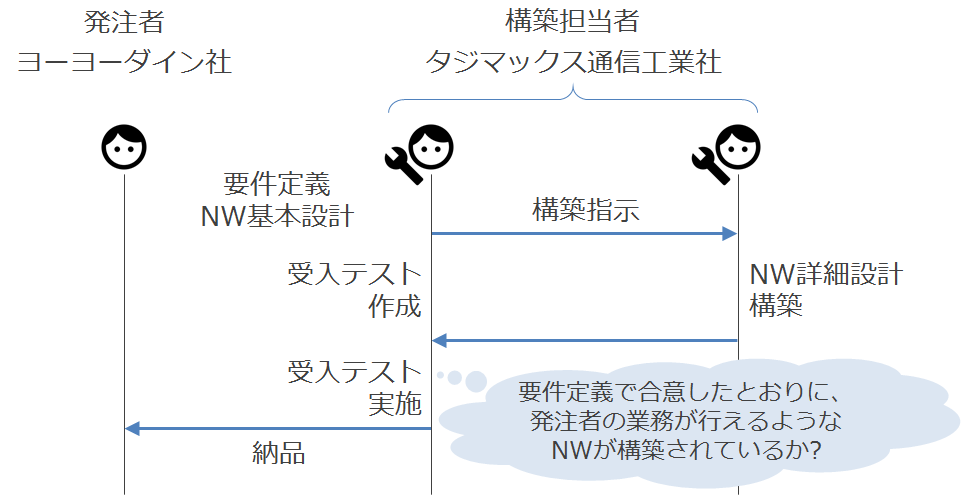
\includegraphics[scale=0.6]{img/poc-situation.png}
 \caption{PoC設定: 登場人物の位置付け}
 \label{fig:poc-situation}
\end{figure}

\subsection{ネットワークに求められる要件}

 \section{環境構成(Target Network)}

  \subsection{論理ネットワーク設計}

\begin{itemize}
 \item L2/L3, Management network (VR/VRFとout-of-band設定)
 \item FWの冗長化設定:
       \begin{itemize}
        \item active/passive, passiveはパケット転送しない
        \item tcp session state を同期する
        \item 状態監視するインタフェースの設定、自動復旧設定とする
       \end{itemize}
 \item FWのフィルタ設定:
       \begin{itemize}
        \item 原則L3/L4でのフィルタ
        \item tcp state をみる
        \item DNSについてはL7(DPI)でフィルタする
       \end{itemize}
\end{itemize}

\begin{figure}[h]
 \centering
 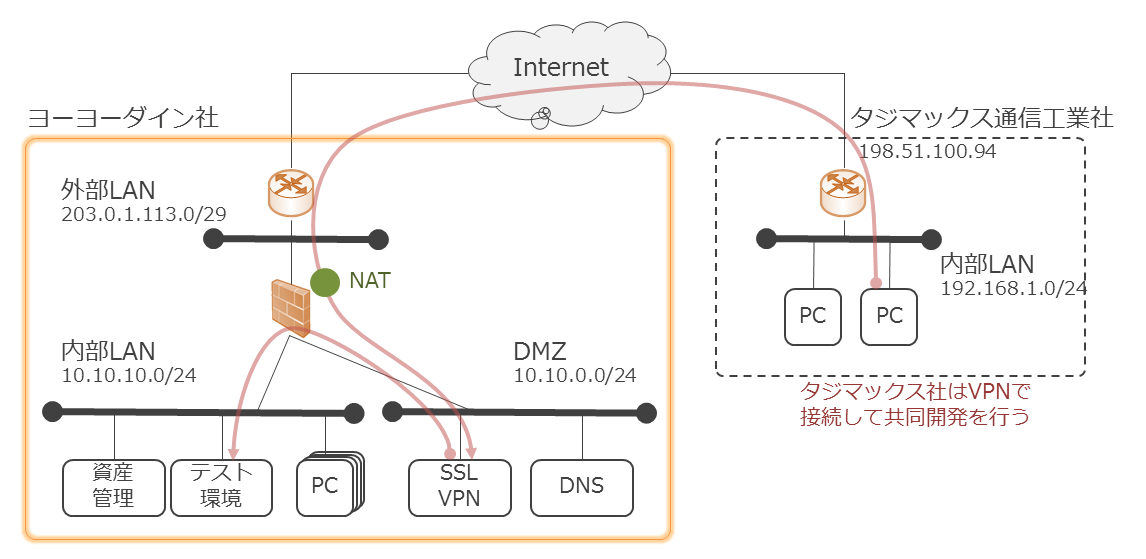
\includegraphics[scale=0.55]{img/poc-env-logical.png}
 \caption{PoC環境: 論理構成図}
 \label{fig:poc-env-logical}
\end{figure}

  \subsection{通信要件}

\begin{landscape}
 \begin{table}[h]
  \centering
  \caption{PoC 通信要件(ヨーヨーダイン社内部セグメント起点)}
  % No.1-12
  \label{tab:poc-requires-yo-int}
  \begin{threeparttable}
   \begin{tabularx}{\linewidth}{c|X|X|X|X|X|X|X}
\hline
No. & ポリシ & アプリケーション & \multicolumn{2}{|l|}{Source IP} & \multicolumn{2}{l|}{Destination IP} & Destination Port \\
\hline
\hline
1 & PC→開発環境 & AP1アクセス & PC & 10.10.10.0/24 & 資産管理サーバ & 10.10.10.1 & tcp/11000 \\ \hline
2 & PC→開発環境 & AP2アクセス & PC & 10.10.10.0/24 & テスト環境サーバ & 10.10.10.2 & tcp/23 \\ \hline
3 & PC→開発環境 & AP3アクセス & PC & 10.10.10.0/24 & テスト環境サーバ & 10.10.10.2 & tcp/13000 \\ \hline
4 & PC→開発環境 & サーバ管理: ssh & PC & 10.10.10.0/24 & 資産管理サーバ & 10.10.10.1 & tcp/22,80,443 \\ \hline
5 & PC→開発環境 & サーバ管理: ssh & PC & 10.10.10.0/24 & テスト環境サーバ & 10.10.10.2 & tcp/22,80,443 \\ \hline
6 & PC→DNSサーバ & DNS Query & PC & 10.10.10.0/24 & DNSサーバ & 10.10.0.10 & tcp,udp/53 \\ \hline
7 & PC→Internet & Web browsing & PC & 10.10.10.0/24 & Internet & ANY & tcp 80,443 \\ \hline
8 & PC→Internet & NTP Query & PC & 10.10.10.0/24 & Internet & ANY & udp/123 \\ \hline
9 & PC→DNSサーバ & 応答確認: ping/traceroute & PC & 10.10.10.0/24 & DMZ & 10.10.0/24 & icmp \\ \hline
10 & PC→Internet & 応答確認: ping/traceroute & PC & 10.10.10.0/24 & Internet & ANY & icmp \\ \hline
11 & PC→DNSサーバ & サーバ管理: ssh & PC & 10.10.10.0/24 & DNSサーバ & 10.10.0.10 & tcp/22 \\ \hline
12 & PC→SSLVPNサーバ & サーバ管理: ssh, webui & PC & 10.10.10.0/24 & SSLVPNサーバ & 10.10.0.11 & tcp/22,80,443 \\ \hline
   \end{tabularx}
   \begin{tablenotes}
    \footnotesize
    \item ヨ社: ヨーヨーダイン社
    \item タ社: タジマックス通信工業社
   \end{tablenotes}
  \end{threeparttable}
 \end{table}
\end{landscape}

\begin{landscape}
 \begin{table}[h]
  \centering
  \caption{PoC 通信要件(ヨーヨーダイン社DMZセグメント起点)}
  % No.13-24
  \label{tab:poc-requires-yo-dmz}
  \begin{threeparttable}
   \begin{tabularx}{\linewidth}{c|X|X|X|X|X|X|X}
\hline
No. & ポリシ & アプリケーション & \multicolumn{2}{|l|}{Source IP} & \multicolumn{2}{l|}{Destination IP} & Destination Port \\
\hline
\hline
13 & DMZ→Internet & package update (web) & DMZ内サーバ & 10.10.0.0/25 & Internet & ANY & tcp/80,443 \\ \hline
14 & DNSサーバ→DNS Query & 上位DNSへのクエリ & DNSサーバ & 10.10.0.10 & Internet & ANY & tcp,udp/53 \\ \hline
15 & DMZ→DNSサーバ & DNS Query & DMZ内サーバ & 10.10.0.0/25 & DNSサーバ & 10.10.0.10 & tcp,udp/53 \\ \hline
16 & DMZ→NTP & NTP Query & DMZ内サーバ & 10.10.0.0/25 & Internet & ANY & udp/123 \\ \hline
17 & PC→DNSサーバ & ヨ社内部 & PC & 10.10.10.0/24 & DNSサーバ & 10.10.0.10 & tcp,udp/53 \\ \hline
18 & PC→DMZ & サーバ管理: ssh & PC & 10.10.10.0/24 & DMZ内サーバ & 10.10.0.0/25 & tcp/22,80,443 \\ \hline
19 & VPNPOOL→開発環境 & AP1アクセス & DMZ VPN Pool & 10.10.0.128/25 & 資産管理サーバ & 10.10.10.1 & tcp/11000 \\ \hline
20 & VPNPOOL→開発環境 & AP2アクセス & DMZ VPN Pool & 10.10.0.128/25 & テスト環境サーバ & 10.10.10.2 & tcp/23 \\ \hline
21 & VPNPOOL→開発環境 & AP3アクセス & DMZ VPN Pool & 10.10.0.128/25 & テスト環境サーバ & 10.10.10.2 & tcp/13000 \\ \hline
22 & DMZ→Internet & 応答確認: ping/traceroute & DMZ内サーバ & 10.10.0.0/25 & Internet & ANY & icmp \\ \hline
23 & DMZ→ヨ社内部 & 応答確認: ping/traceroute & ヨ社内部 & 10.10.10.0/24 & DMZ内サーバ & 10.10.0.0/25 & icmp \\ \hline
24 & ヨ社内部→DMZ & 応答確認: ping/traceroute & DMZ内サーバ & 10.10.0.0/25 & ヨ社内部 & 10.10.10.0/24 & icmp \\ \hline
   \end{tabularx}
   \begin{tablenotes}
    \footnotesize
    \item ヨ社: ヨーヨーダイン社
    \item タ社: タジマックス通信工業社
   \end{tablenotes}
  \end{threeparttable}
 \end{table}
\end{landscape}

\begin{landscape}
 \begin{table}[h]
  \centering
  \caption{PoC 通信要件(Internet/タジマックス社セグメント起点)}
  % No.25-28(Internet), No.29-30(タ社)
  \label{tab:poc-requires-etc}
  \begin{threeparttable}
   \begin{tabularx}{\linewidth}{c|X|X|X|X|X|X|X}
\hline
No. & ポリシ & アプリケーション & \multicolumn{2}{|l|}{Source IP} & \multicolumn{2}{l|}{Destination IP} & Destination Port \\
\hline
\hline
26 & Internet→外部 & 応答確認: ping/traceroute & Internet & ANY & Router & 203.0.113.1 & icmp \\ \hline
27 & Internet→外部 & 応答確認: ping/traceroute & Internet & ANY & Firewall & 203.0.113.2 & icmp \\ \hline
28 & 外部→Internet & 応答確認: ping/traceroute & ヨ社外部 & 203.0.113.0/29 & Internet & ANY & icmp \\ \hline
29 & PC→ヨ社VPN & SSLVPN & タ社(Global) & 198.51.100.94 & SSLVPNサーバ & 203.0.113.5 & tcp/80,443 \\ \hline
30 & PC→ヨ社VPN & 応答確認: ping/traceroute & タ社(Global) & 198.51.100.94 & SSLVPNサーバ & 203.0.113.5 & icmp \\ \hline
   \end{tabularx}
   \begin{tablenotes}
    \footnotesize
    \item ヨ社: ヨーヨーダイン社
    \item タ社: タジマックス通信工業社
   \end{tablenotes}
  \end{threeparttable}
 \end{table}
\end{landscape}

  \subsection{物理ネットワーク設計}

\begin{figure}[h]
 \centering
 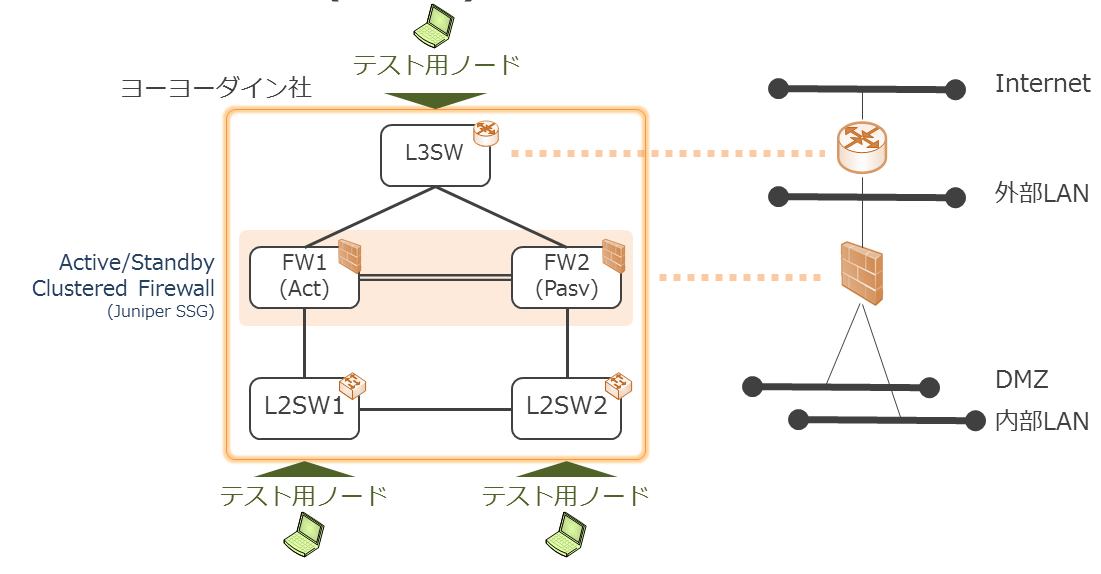
\includegraphics[scale=0.55]{img/poc-env-physical.png}
 \caption{PoC環境: 物理構成図(概要)}
 \label{fig:poc-env-physical}
\end{figure}

\section{環境構成(NetTester)}

\begin{itemize}
 \item Tester Set について
 \item 構成図 \url{https://drive.google.com/open?id=0B2eRR_JxYJA5Nm1VbzBnR1FQMUk}
 \item IPアドレス表 \url{https://drive.google.com/open?id=1v0ecUjUql3cxVMP8gvLyq4T9PEIeUeyMT_-9YrR4l0A}
 \item Syslogについて
\end{itemize}

\begin{landscape}
 \begin{figure}[h]
  \centering
  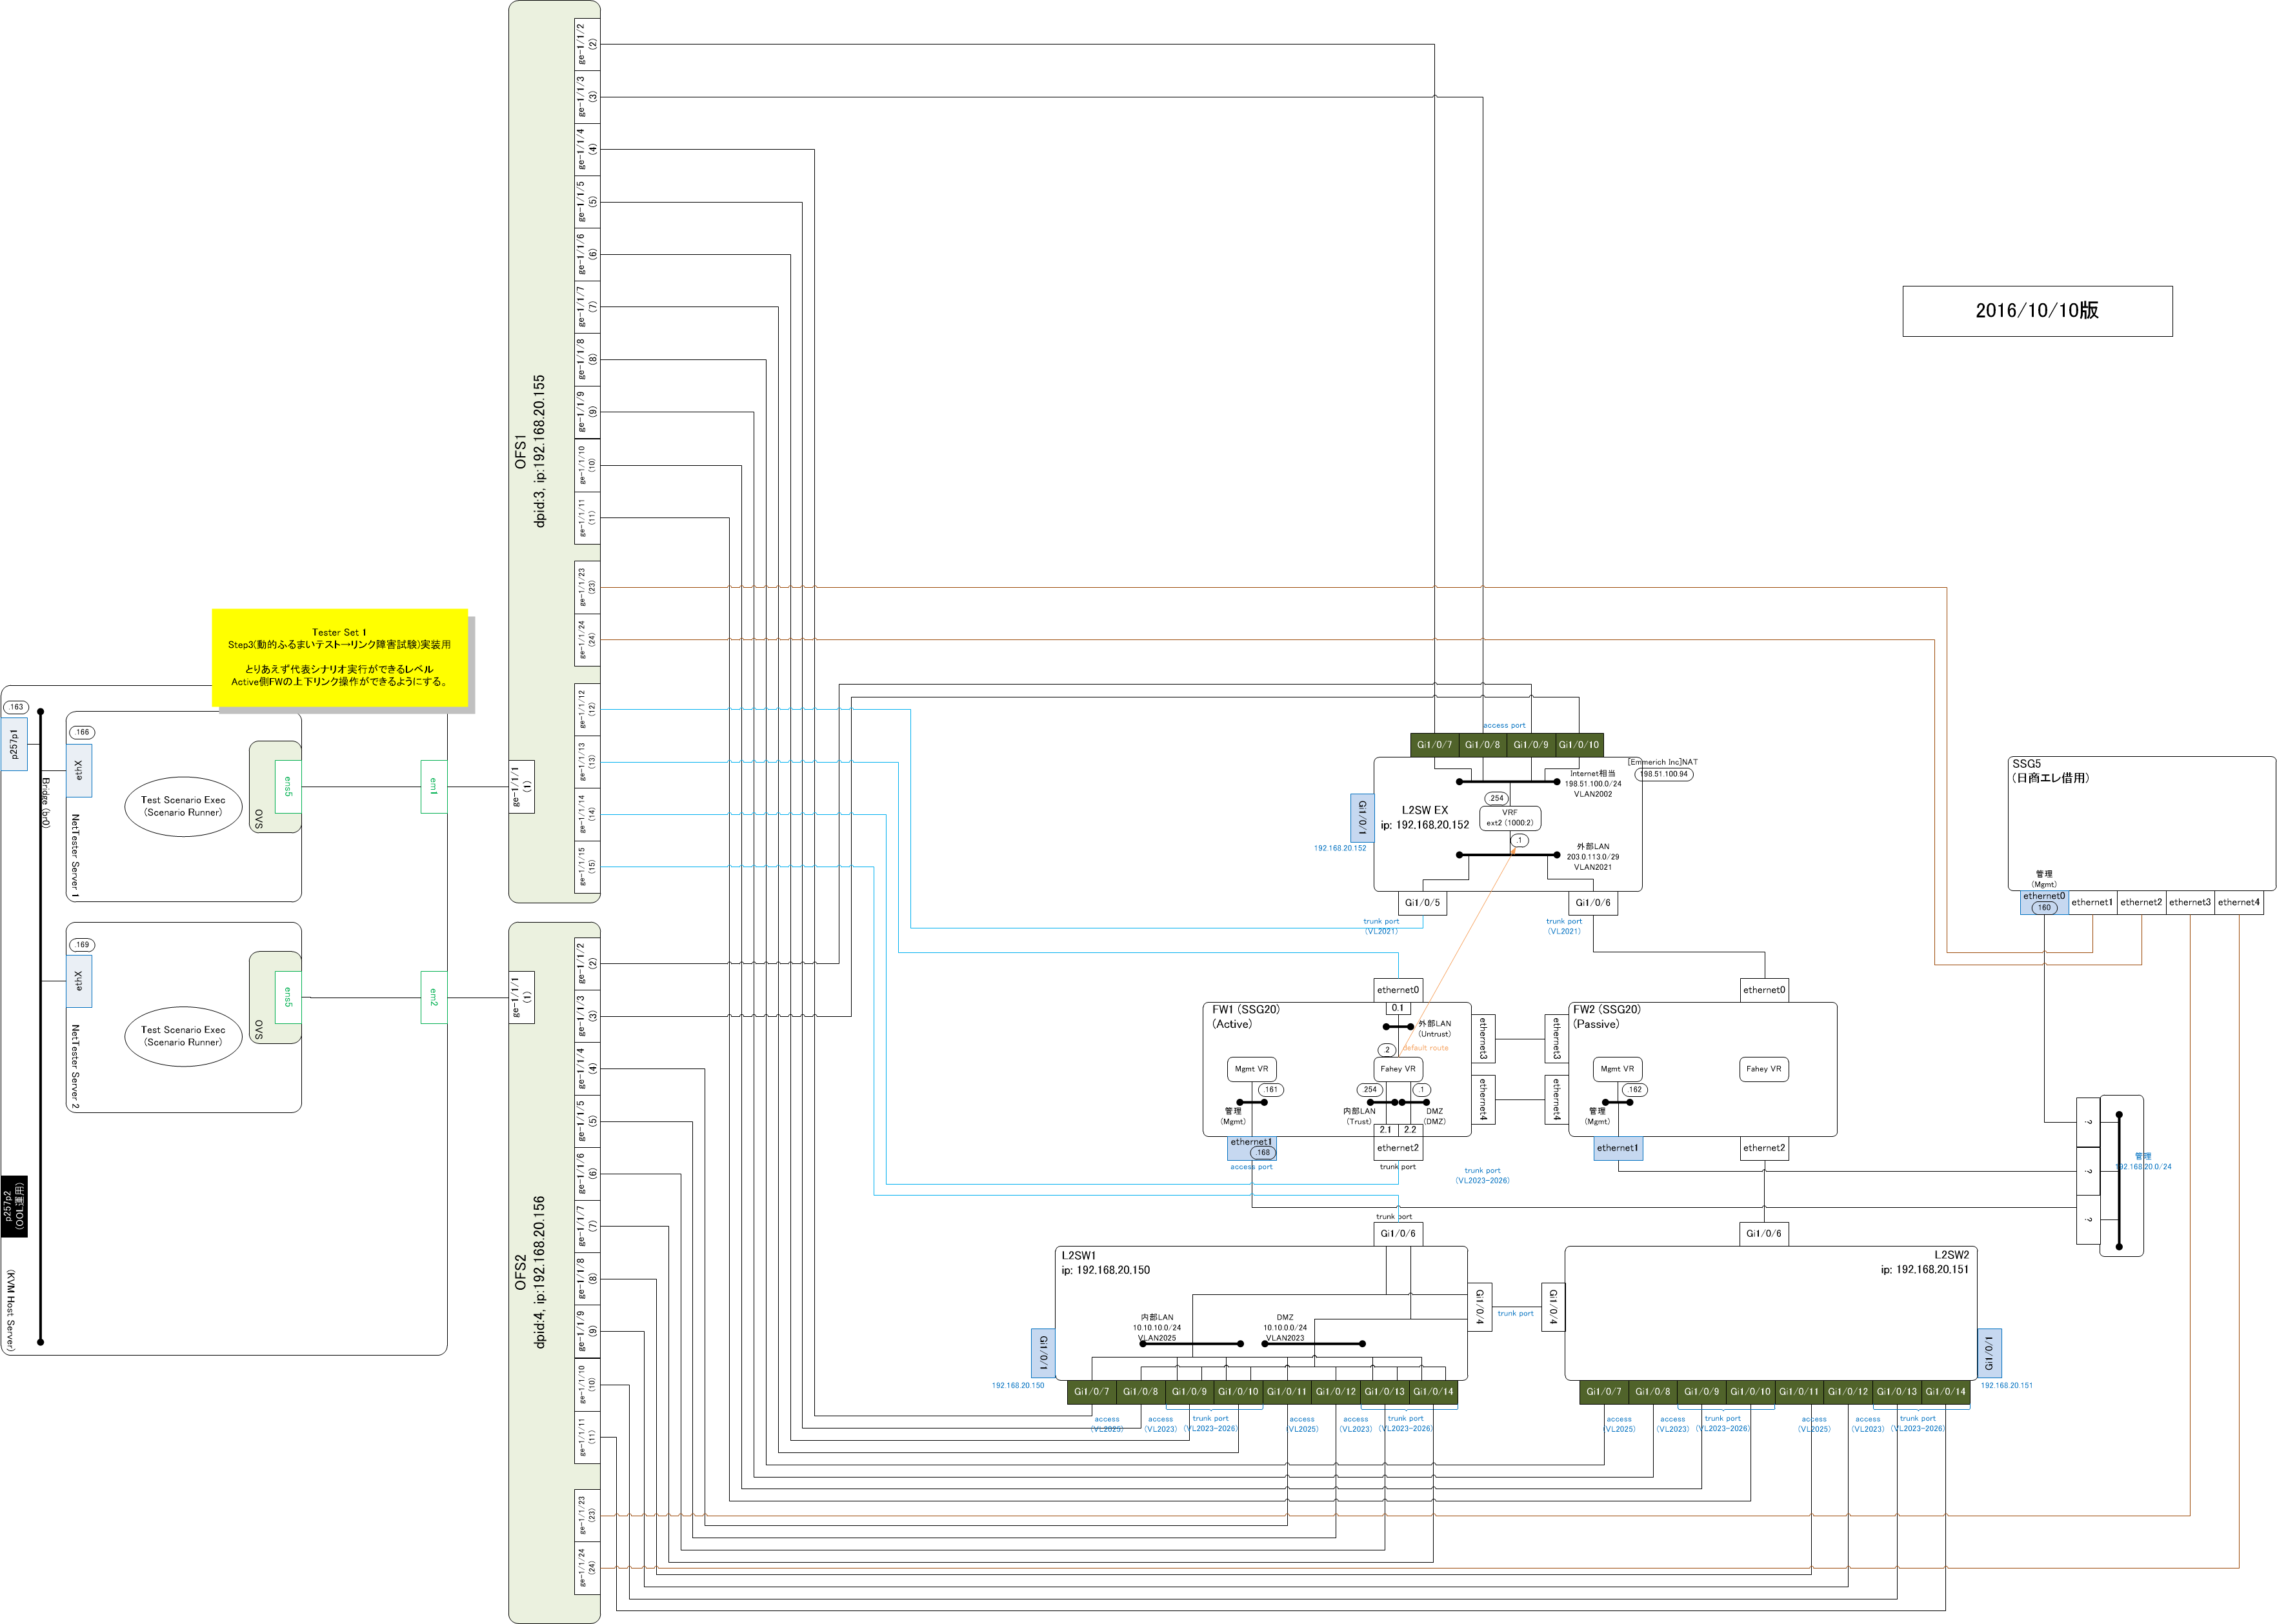
\includegraphics[scale=0.225]{img/poc-env-physical-detail.png}
  \caption{PoC環境: 物理構成図(詳細)}
  \label{fig:poc-env-physical-detail}
 \end{figure}
\end{landscape}

\section{静的なテスト}


\begin{itemize}
 \item 実装
       \begin{itemize}
        \item Step2テスト業務で気づいたことをまとめる – NetTester \url{https://3.basecamp.com/3088280/buckets/867009/todos/260220903}
       \end{itemize}
 \item 結果: 実際に発見できたトラブルや設定ミスなどをあげる。

       \begin{itemize}
        \item Teardown関連
              \begin{itemize}
               \item 原因切り分けメモ (muraki) – NetTester \url{https://3.basecamp.com/3088280/buckets/867009/documents/217782147}
               \item 調査: テスト環境でシナリオ実行すると2回目以降でコケる – NetTester \url{https://3.basecamp.com/3088280/buckets/867009/todos/218486066}
              \end{itemize}
        \item Target Network の設定不備の発見
              \begin{itemize}
               \item DNSのテスト作る – NetTester \url{https://3.basecamp.com/3088280/buckets/867009/todos/301325453}
               \item 通信要件\#10 A社内PC→インターネットの疎通確認(ICMP) – NetTester \url{https://3.basecamp.com/3088280/buckets/867009/todos/233175867}
               \item 通信要件\#29 B社PC→DMZ内のVPNサーバの疎通確認(SSLVPN) – NetTester \url{https://3.basecamp.com/3088280/buckets/867009/todos/233178490}
              \end{itemize}
       \end{itemize}
\end{itemize}

\section{動的なテスト}

障害試験シナリオを書く – NetTester \url{https://3.basecamp.com/3088280/buckets/867009/todos/238169066}

\begin{figure}[h]
 \centering
 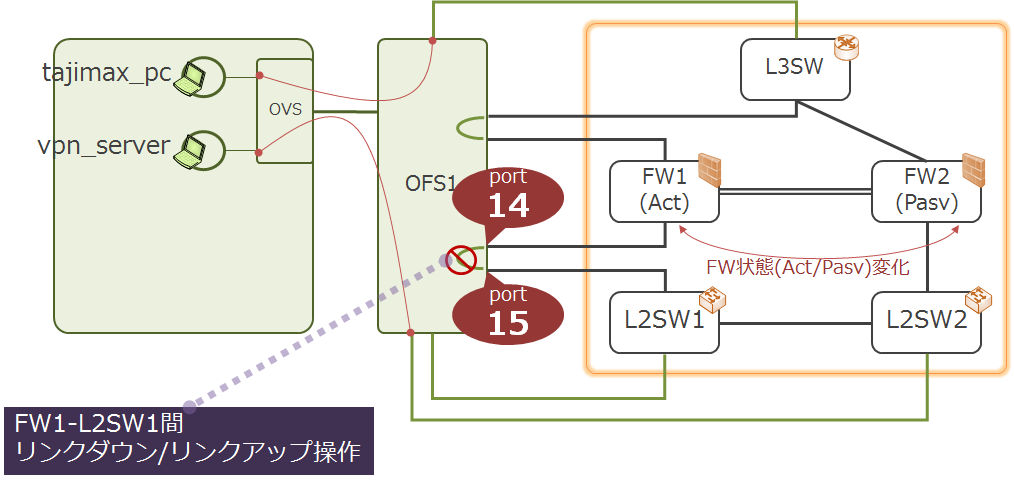
\includegraphics[scale=0.6]{img/poc-env-linkdown.png}
 \caption{PoC環境: NetTesterによるリンクダウン操作}
 \label{fig:poc-env-linkdown}
\end{figure}

\begin{itemize}
 \item 実装 (NAT IPの変更とかデモの話をどこまで含めるか?)
 \item 結果
\end{itemize}

\section{シナリオテスト実装における検討ポイント}

\subsection{Teardown処理}

\begin{itemize}
 \item Target network の状態
       \begin{itemize}
        \item ARP Table のクリア
        \item NAT Table のクリア
        \item Firewall の active/standby (自動復旧にしているのでとくにいれていない)
       \end{itemize}
 \item Netns の /etc 配下のクリア
       \begin{itemize}
        \item 自作echoサーバーで通信開始時に10秒のラグが起きる問題 – NetTester \url{https://3.basecamp.com/3088280/buckets/867009/todos/274457003}
       \end{itemize}
 \item 物理OFSのflow tableのクリア (まだやれてない)
\end{itemize}

\subsection{テストシナリオのサイズ}

シナリオサイズの目安、シナリオ分割の目安 (step3 test つくっているときに
分割するって話になった理由は?)

\section{PoC結果}

結果まとめ

%%% Local Variables:
%%% mode: yatex
%%% TeX-master: "main.tex"
%%% End:
